\documentclass[conference]{IEEEtran}
\usepackage[utf8]{inputenc}
\usepackage[spanish,es-tabla]{babel}
\usepackage{amsmath,amssymb,amsfonts}
\usepackage{graphicx}
\usepackage{cite}
\usepackage{booktabs}
\usepackage{microtype}
\usepackage{url}
\usepackage{bm}
\usepackage{listings}
\usepackage{xcolor}
\usepackage{subcaption}

% Configuracion de listings para codigo MATLAB
\definecolor{codegreen}{rgb}{0,0.5,0}
\definecolor{codegray}{rgb}{0.5,0.5,0.5}
\definecolor{codepurple}{rgb}{0.58,0,0.82}
\definecolor{backcolour}{rgb}{0.97,0.97,0.97}

\lstdefinestyle{matlabstyle}{
    backgroundcolor=\color{backcolour},   
    commentstyle=\color{codegreen}\itshape,
    keywordstyle=\color{blue}\bfseries,
    numberstyle=\tiny\color{codegray},
    stringstyle=\color{codepurple},
    basicstyle=\ttfamily\scriptsize,
    breakatwhitespace=false,         
    breaklines=true,                 
    captionpos=b,                    
    keepspaces=true,                 
    numbers=left,                    
    numbersep=4pt,                  
    showspaces=false,                
    showstringspaces=false,
    showtabs=false,                  
    tabsize=2,
    frame=single,
    rulecolor=\color{codegray}
}
\lstset{style=matlabstyle}

\begin{document}

\title{Modelado Teórico y Simulación en MATLAB de Procesos Estocásticos: Clasificación, Estacionariedad en Sentido Amplio y Ergodicidad en Sistemas de Telecomunicaciones}

\author{
\IEEEauthorblockN{Franco Arturo Gutiérrez Ccolqque, Fernando Gaimez Ollachica, Zaul Francisco Uturunco Cuela,}
\IEEEauthorblockN{Fernando Josue Castro Quispe, Benjamin Eduardo Quispe Flores}
\IEEEauthorblockA{\textit{Escuela Profesional de Ingeniería en Telecomunicaciones} \\
\textit{Universidad Nacional de San Agustín de Arequipa (UNSA)}\\
Arequipa, Perú \\
Curso: Métodos Matemáticos 2 (1702228) --- Grupo 02}
}

\maketitle

\begin{abstract}
Este artículo presenta una investigación analítica y computacional sobre los fundamentos de los procesos estocásticos orientada a la ingeniería en telecomunicaciones, abordando su clasificación formal, las condiciones de estacionariedad y la propiedad de ergodicidad. Se modela rigurosamente una señal portadora sinusoidal con fase aleatoria uniformemente distribuida, representativa de osciladores locales y frentes de onda en canales inalámbricos sin sincronización previa. Mediante simulaciones en MATLAB empleando el método de Monte Carlo, se analiza el comportamiento estadístico de primer y segundo orden para distintos tamaños de ensamble. Los resultados demuestran empíricamente que la media de conjunto es nula y que la autocorrelación depende exclusivamente del retardo temporal, satisfaciendo estrictamente la estacionariedad en sentido amplio. Asimismo, se comprueba la ergodicidad en media y en autocorrelación contrastando promedios de conjunto frente a promedios temporales sobre una única trayectoria continua. Finalmente, se examina un contraejemplo no estacionario con envolvente modulada linealmente en el tiempo, demostrando analítica y numéricamente la ruptura de la invarianza temporal en la varianza y la autocorrelación. Todos los experimentos computacionales validan con alta precisión la teoría estadística con errores relativos inferiores al 0.02\%.
\end{abstract}

\begin{IEEEkeywords}
Procesos estocásticos, estacionariedad en sentido amplio (WSS), ergodicidad, ensamble de trayectorias, autocorrelación, telecomunicaciones, simulación Monte Carlo.
\end{IEEEkeywords}

\section{Introducción}
En la ingeniería moderna de telecomunicaciones, la transmisión y recepción de información electromagnética está sujeta de manera intrínseca a fenómenos aleatorios. Fuentes térmicas en componentes resistivos de radiofrecuencia (ruido de Johnson-Nyquist), retardos de propagación multicamino impredecibles en el canal móvil, fluctuaciones en la frecuencia y fase instantánea de osciladores locales, y la propia naturaleza de la información digital transmitida impiden modelar las señales mediante funciones temporales determinísticas aisladas \cite{leon2008, proakis2008}.

Un oscilador de portadora no sincronizado en el receptor de un sistema inalámbrico constituye un ejemplo canónico: la amplitud y la frecuencia nominal pueden conocerse de antemano, pero la fase relativa observada en la antena receptora depende de la distancia física al transmisor (múltiplos no enteros de la longitud de onda $\lambda = c / f_0$) y del instante de conmutación. Esta incertidumbre fundamental exige recurrir a la teoría de probabilidades y, en particular, al concepto de \textit{procesos estocásticos} para describir familias completas de señales posibles.

El objetivo primordial del presente trabajo es formular de manera rigurosa la teoría de procesos estocásticos, formalizar su taxonomía bidimensional (tiempo y estado continuos o discretos), diferenciar analíticamente la estacionariedad estricta de la estacionariedad en sentido amplio (\textit{Wide-Sense Stationarity}, WSS) y fundamentar el principio de ergodicidad. Asimismo, se implementa en MATLAB una plataforma computacional de simulación para modelar un ensamble de realizaciones de portadora con fase aleatoria uniforme $X(t) = A\cos(2\pi f_0 t + \Theta)$, verificando la invarianza temporal de la media y la dependencia de la autocorrelación únicamente del retardo $\tau$. Se compara además el promedio de conjunto con el promedio temporal de una sola trayectoria para validar la ergodicidad, y se somete a prueba un contraejemplo no estacionario para analizar las causas físicas y matemáticas de la no estacionariedad.

\section{Marco Teórico}

\subsection{Definición de Proceso Estocástico}
Un proceso estocástico $\{X(t, \zeta), t \in \mathcal{T}, \zeta \in \Omega\}$ es formalmente una colección indexada de variables aleatorias definidas sobre un espacio de probabilidad común $(\Omega, \mathcal{F}, P)$, donde $\mathcal{T} \subseteq \mathbb{R}$ representa el conjunto de índices (típicamente el tiempo) y $\Omega$ denota el espacio muestral \cite{papoulis2002}. Dependiendo de las fijaciones de sus argumentos, un proceso estocástico admite cuatro interpretaciones fundamentales:
\begin{enumerate}
    \item Para un tiempo fijo $t_0 \in \mathcal{T}$ y $\zeta$ variable, $X(t_0, \zeta)$ es una \textbf{variable aleatoria} ordinaria.
    \item Para un evento muestral fijo $\zeta_0 \in \Omega$ y $t \in \mathcal{T}$ variable, $X(t, \zeta_0)$ es una función determinística del tiempo, denominada \textbf{realización}, trayectoria o camino muestral (\textit{sample path}).
    \item Para $t_0$ y $\zeta_0$ fijos simultáneamente, $X(t_0, \zeta_0)$ es un \textbf{número real} específico.
    \item Para $t$ y $\zeta$ variables, representa la totalidad del \textbf{proceso estocástico} (el ensamble de todas las trayectorias posibles).
\end{enumerate}

\subsection{Clasificación de Procesos Estocásticos}
En función de la cardinalidad y continuidad del dominio temporal $\mathcal{T}$ y del espacio de estados $\mathcal{S}$ (valores asumidos por $X(t)$), los procesos se clasifican en cuatro categorías fundamentales en telecomunicaciones (Tabla~\ref{tab:clasificacion}):

\begin{table}[htbp]
\caption{Clasificación bidimensional de procesos estocásticos en telecomunicaciones.}
\label{tab:clasificacion}
\centering
\resizebox{\columnwidth}{!}{%
\begin{tabular}{p{2.2cm}p{2.5cm}p{3.2cm}}
\toprule
\textbf{Categoría} & \textbf{Espacio $(\mathcal{T}, \mathcal{S})$} & \textbf{Ejemplo en Telecom.} \\
\midrule
Tiempo continuo, estado continuo & $\mathcal{T} = \mathbb{R}, \; \mathcal{S} = \mathbb{R}$ & Voltaje de ruido térmico AWGN $n(t)$, portadora desfasada $X(t)$. \\
Tiempo continuo, estado discreto & $\mathcal{T} = \mathbb{R}, \; \mathcal{S} \subset \mathbb{Z}$ & Conteo de paquetes arribados a un conmutador (Poisson), señal telegráfica. \\
Tiempo discreto, estado continuo & $\mathcal{T} \subset \mathbb{Z}, \; \mathcal{S} = \mathbb{R}$ & Muestras de voz antes de cuantificación, coeficientes de canal $h[n]$. \\
Tiempo discreto, estado discreto & $\mathcal{T} \subset \mathbb{Z}, \; \mathcal{S} \subset \mathbb{Z}$ & Bits transmitidos en banda base $b[n] \in \{0,1\}$, estados de modulación QAM. \\
\bottomrule
\end{tabular}%
}
\end{table}

\subsection{Estacionariedad: Estricta (SSS) vs. Sentido Amplio (WSS)}
La estacionariedad describe la invarianza de las propiedades estadísticas de un proceso frente a desplazamientos en el origen de los tiempos \cite{walpole2012, leon2008}.

\textbf{1) Estacionariedad en Sentido Estricto (SSS):} Un proceso $X(t)$ es estacionario en sentido estricto si su función de distribución acumulada conjunta de cualquier orden finito $k$ es invariante ante un corrimiento temporal arbitrario $\tau \in \mathbb{R}$:
\begin{align}
&F_{X(t_1),\dots,X(t_k)}(x_1,\dots,x_k) \nonumber \\
&\quad = F_{X(t_1+\tau),\dots,X(t_k+\tau)}(x_1,\dots,x_k),
\label{eq:sss}
\end{align}
para todo $k \ge 1$ y todo $\{t_1, \dots, t_k\} \subset \mathcal{T}$.

\textbf{2) Estacionariedad en Sentido Amplio (WSS):} La condición SSS resulta extremadamente difícil de verificar empíricamente en sistemas reales, pues exige conocer las distribuciones conjuntas de orden infinito. En ingeniería de telecomunicaciones se emplea la condición de segundo orden WSS, que impone dos requisitos necesarios y suficientes:
\begin{itemize}
    \item La media de conjunto es constante e independiente del tiempo:
    \begin{equation}
    \mu_X(t) = \mathbb{E}[X(t)] = \mu_X = \text{constante}, \quad \forall t.
    \label{eq:mean_wss}
    \end{equation}
    \item La función de autocorrelación de conjunto depende única y exclusivamente de la diferencia temporal $\tau = t_2 - t_1$:
    \begin{equation}
    R_X(t_1, t_2) = \mathbb{E}[X(t_1) X(t_2)] = R_X(t_2 - t_1) = R_X(\tau).
    \label{eq:rx_wss}
    \end{equation}
    \item Potencia media finita: $\mathbb{E}[X^2(t)] = R_X(0) < \infty$.
\end{itemize}
Todo proceso SSS de segundo orden con varianza finita es WSS. El recíproco no se cumple en general, salvo en la familia de procesos gaussianos, donde los dos primeros momentos determinan completamente la densidad de probabilidad conjunta \cite{papoulis2002}. En el ámbito de las telecomunicaciones, la formulación WSS es fundamental: constituye la hipótesis sobre la cual Bello formalizó la caracterización de canales de propagación móviles dispersivos e incorrelados (WSSUS) \cite{bello1963}, estándar universal para comunicaciones celulares 4G y 5G.

\subsection{Ergodicidad en Procesos WSS}
En la práctica de laboratorio o en receptores físicos, no es factible acceder a un conjunto infinito de realizaciones simultáneas $\zeta_m$. En su lugar, el ingeniero captura una \textit{única} señal temporal $x(t)$ de longitud finita o prolongada. Un proceso estocástico es \textbf{ergódico} si sus promedios estadísticos de conjunto pueden calcularse a partir de promedios temporales ejecutados sobre una única trayectoria cualquiera cuando el intervalo de observación tiende a infinito \cite{leon2008}:

\textbf{1) Ergodicidad en la media:}
\begin{equation}
\langle x(t) \rangle = \lim_{T \to \infty} \frac{1}{2T} \int_{-T}^{T} x(t) \, dt = \mathbb{E}[X(t)] = \mu_X \quad \text{c.s.}
\label{eq:erg_mean}
\end{equation}
donde ``c.s.'' denota convergencia con probabilidad 1 (casi seguro).

\textbf{2) Ergodicidad en la autocorrelación:}
\begin{equation}
\mathcal{R}_x(\tau) = \lim_{T \to \infty} \frac{1}{2T} \int_{-T}^{T} x(t) x(t+\tau) \, dt = R_X(\tau) \quad \text{c.s.}
\label{eq:erg_rx}
\end{equation}

\subsection{Deducción Analítica del Modelo Sinusoidal con Fase Aleatoria}
Considérese el proceso estocástico continuo:
\begin{equation}
X(t) = A \cos(2\pi f_0 t + \Theta),
\label{eq:modelo_sin}
\end{equation}
donde la amplitud $A > 0$ y la frecuencia de portadora $f_0 > 0$ son constantes determinísticas, y la fase $\Theta$ es una variable aleatoria continua con distribución uniforme en el intervalo $[0, 2\pi)$, cuya función de densidad de probabilidad (fdp) es:
\begin{equation}
f_\Theta(\theta) = \begin{cases}
\frac{1}{2\pi}, & 0 \le \theta < 2\pi, \\
0, & \text{en otro caso.}
\end{cases}
\end{equation}

\textbf{1) Esperanza matemática (media de conjunto):}
\begin{equation}
\mu_X(t) = \mathbb{E}[X(t)] = \int_{0}^{2\pi} A \cos(2\pi f_0 t + \theta) \frac{1}{2\pi} \, d\theta.
\end{equation}
Efectuando la integración directa sobre un periodo completo $2\pi$:
\begin{equation}
\mu_X(t) = \frac{A}{2\pi} \Big[ \sin(2\pi f_0 t + \theta) \Big]_0^{2\pi} = 0, \quad \forall t.
\label{eq:mu_teorica}
\end{equation}
Por tanto, la media de conjunto es estrictamente cero para todo instante de tiempo, cumpliendo la primera condición WSS.

\textbf{2) Función de autocorrelación de conjunto:}
\begin{align}
R_X(t_1, t_2) &= \mathbb{E}\big[ X(t_1) X(t_2) \big] \nonumber \\
&= \mathbb{E}\big[ A^2 \cos(2\pi f_0 t_1 + \Theta) \cos(2\pi f_0 t_2 + \Theta) \big].
\end{align}
Aplicando la identidad trigonométrica del producto de cosenos, $\cos(\alpha)\cos(\beta) = \frac{1}{2}[\cos(\alpha - \beta) + \cos(\alpha + \beta)]$, con $\alpha = 2\pi f_0 t_2 + \Theta$ y $\beta = 2\pi f_0 t_1 + \Theta$:
\begin{align}
X(t_1)X(t_2) &= \frac{A^2}{2} \cos(2\pi f_0 (t_2 - t_1)) \nonumber \\
&\quad + \frac{A^2}{2} \cos(2\pi f_0 (t_1 + t_2) + 2\Theta).
\end{align}
Tomando la esperanza respecto a $\Theta$:
\begin{align}
&\mathbb{E}\big[\cos(2\pi f_0 (t_1 + t_2) + 2\Theta)\big] \nonumber \\
&\quad = \int_0^{2\pi} \frac{\cos(2\pi f_0 (t_1 + t_2) + 2\theta)}{2\pi} \, d\theta \nonumber \\
&\quad = \frac{1}{2\pi} \left[ \frac{\sin(2\pi f_0(t_1+t_2) + 2\theta)}{2} \right]_0^{2\pi} = 0.
\end{align}
Por consiguiente, el segundo término se anula idénticamente, resultando:
\begin{equation}
R_X(t_1, t_2) = \frac{A^2}{2} \cos(2\pi f_0 (t_2 - t_1)).
\end{equation}
Definiendo el retardo $\tau = t_2 - t_1$:
\begin{equation}
R_X(\tau) = \frac{A^2}{2} \cos(2\pi f_0 \tau).
\label{eq:rx_teorica}
\end{equation}
Dado que $\mu_X(t) = 0$ es constante y $R_X(t_1, t_2)$ no depende de $t_1$ ni de $t_2$ de forma individual sino exclusivamente de su desfase $\tau$, \textbf{el proceso es WSS}. La potencia media del proceso corresponde al valor en el origen:
\begin{equation}
P_X = R_X(0) = \frac{A^2}{2}.
\label{eq:potencia_teorica}
\end{equation}

\textbf{3) Densidad Espectral de Potencia (DEP):}
En virtud del teorema de Wiener-Khinchin, la DEP es la transformada de Fourier de la función de autocorrelación:
\begin{equation}
S_X(f) = \mathcal{F}\{R_X(\tau)\} = \frac{A^2}{4} \big[ \delta(f - f_0) + \delta(f + f_0) \big].
\label{eq:dep_teorica}
\end{equation}
La integración de $S_X(f)$ sobre todo el espectro confirma la conservación de potencia: $\int_{-\infty}^{\infty} S_X(f) df = A^2/2 = P_X$.

\textbf{4) Demostración analítica de ergodicidad:}
Para una trayectoria fijada arbitraria $x(t) = A\cos(2\pi f_0 t + \theta_0)$ con fase $\theta_0 \in [0, 2\pi)$:
\begin{equation}
\langle x(t) \rangle = \lim_{T \to \infty} \frac{1}{2T} \int_{-T}^{T} A\cos(2\pi f_0 t + \theta_0) \, dt = 0 = \mathbb{E}[X(t)].
\end{equation}
Asimismo, calculando la correlación temporal:
\begin{align}
\mathcal{R}_x(\tau) &= \lim_{T \to \infty} \frac{1}{2T} \int_{-T}^{T} A^2 \cos(2\pi f_0 t + \theta_0) \nonumber \\
&\qquad\quad \times \cos(2\pi f_0 (t+\tau) + \theta_0) \, dt \nonumber \\
&= \frac{A^2}{2}\cos(2\pi f_0 \tau) \nonumber \\
&\quad + \lim_{T \to \infty} \frac{A^2}{4T} \int_{-T}^{T} \cos(4\pi f_0 t + 2\pi f_0 \tau + 2\theta_0) \, dt \nonumber \\
&= \frac{A^2}{2}\cos(2\pi f_0 \tau) = R_X(\tau).
\label{eq:erg_demostracion}
\end{align}
El término oscilatorio a frecuencia $2f_0$ promedia a cero en el límite, verificando que \textbf{el proceso es estrictamente ergódico tanto en la media como en la autocorrelación}.

\textbf{5) Descomposición Ortogonal en Fase y Cuadratura ($I/Q$):}
En receptores de comunicaciones digitales y radio definida por software (SDR), las señales sinusoidales se descomponen habitualmente en dos ramas en cuadratura en banda base mediante la identidad de suma de ángulos:
\begin{align}
X(t) &= A \cos(2\pi f_0 t + \Theta) \nonumber \\
&= \underbrace{A \cos\Theta}_{X_I} \cos(2\pi f_0 t) - \underbrace{A \sin\Theta}_{X_Q} \sin(2\pi f_0 t),
\label{eq:descomposicion_iq}
\end{align}
donde las amplitudes $X_I = A\cos\Theta$ y $X_Q = A\sin\Theta$ son variables aleatorias continuas. Sus momentos estadísticos satisfacen:
\begin{itemize}
    \item Media nula: $\mathbb{E}[X_I] = \mathbb{E}[X_Q] = 0$.
    \item Varianzas idénticas:
    \begin{equation}
    \mathbb{E}[X_I^2] = \frac{A^2}{2\pi} \int_0^{2\pi} \cos^2\theta \, d\theta = \frac{A^2}{2} = \mathbb{E}[X_Q^2].
    \end{equation}
    \item Incorrelación mutua:
    \begin{equation}
    \mathbb{E}[X_I X_Q] = \frac{A^2}{2\pi} \int_0^{2\pi} \cos\theta \sin\theta \, d\theta = 0.
    \end{equation}
\end{itemize}
Esta ortogonalidad estadística confirma que la energía de la portadora se distribuye simétricamente entre las fases $I$ y $Q$ sin interferencia mutua, base indispensable para esquemas QPSK, QAM y OFDM \cite{proakis2008}.

\section{Desarrollo y Metodología Experimental en MATLAB}

\subsection{Parámetros del Sistema y Criterio de Muestreo}
Para la implementación computacional se seleccionaron parámetros representativos de una señal de frecuencia intermedia (IF) en telecomunicaciones:
\begin{itemize}
    \item Amplitud de pico: $A = 2.0\text{ V}$ (potencia normalizada $P_X = A^2/2 = 2.0\text{ W}$).
    \item Frecuencia fundamental: $f_0 = 1000\text{ Hz}$ ($1\text{ kHz}$), con periodo $T_0 = 1\text{ ms}$.
    \item Frecuencia de muestreo: $f_s = 20000\text{ Hz}$ ($20\text{ kSa/s}$). Cumple con creces el criterio de Nyquist-Shannon ($f_s = 20 f_0 > 2 f_0$), proporcionando una resolución temporal de 20 muestras discretas por ciclo sinusoidal ($\Delta t = 50\,\mu\text{s}$).
    \item Ventana de observación de conjunto: $T_{\text{obs}} = 5\text{ ms}$ (5 ciclos completos, $N = 101$ muestras temporales).
    \item Ventana para análisis de ergodicidad temporal: $T_{\text{long}} = 1.0\text{ s}$ ($1000$ ciclos de portadora, $N_{\text{long}} = 20001$ muestras), asegurando la convergencia asintótica del estimador temporal.
\end{itemize}

\subsection{Estimadores Estadísticos Discretos}
El ensamble se modela como una matriz bidimensional $\mathbf{X} \in \mathbb{R}^{M \times N}$, donde cada fila representa una realización temporal independiente $x_m(t_n) = A\cos(2\pi f_0 t_n + \Theta_m)$, generada mediante variables pseudoaleatorias $\Theta_m \sim U(0, 2\pi)$ con semilla fijada (\texttt{seed = 202608}).

\textbf{1) Estimador de media de conjunto:}
\begin{equation}
\hat{\mu}_X(t_n) = \frac{1}{M} \sum_{m=1}^{M} X_m(t_n).
\end{equation}

\textbf{2) Estimador de varianza de conjunto:}
\begin{equation}
\hat{\sigma}_X^2(t_n) = \frac{1}{M - 1} \sum_{m=1}^{M} \big( X_m(t_n) - \hat{\mu}_X(t_n) \big)^2.
\end{equation}

\textbf{3) Matriz de autocorrelación de conjunto:}
\begin{equation}
\hat{R}_X(t_i, t_j) = \frac{1}{M} \sum_{m=1}^{M} X_m(t_i) X_m(t_j) = \frac{1}{M} [\mathbf{X}^T \mathbf{X}]_{i,j}.
\end{equation}
La extracción de $\hat{R}_X(\tau)$ para un retardo discreto $k \Delta t$ se efectúa promediando las diagonales paralelas a la diagonal principal de la matriz $\hat{R}_X(t_i, t_j)$, verificando si existe invariancia ante la elección del instante de referencia temporal.

\textbf{4) Estimador insesgado de correlación temporal:}
Para una sola trayectoria $x[n]$ evaluada sobre $N_{\text{long}}$ muestras, el estimador insesgado se calcula mediante:
\begin{equation}
\hat{\mathcal{R}}_x[k] = \frac{1}{N_{\text{long}} - |k|} \sum_{n=1}^{N_{\text{long}} - |k|} x[n] x[n + k].
\end{equation}

\subsection{Estructura Modular de los Scripts}
El código en MATLAB se estructuró en cinco módulos independientes para garantizar trazabilidad, modularidad y reproducibilidad:
\begin{itemize}
    \item \texttt{config\_parametros.m}: Centraliza todos los parámetros físicos, vectores temporales y rutas de exportación.
    \item \texttt{generar\_proceso\_sinusoidal.m}: Genera la matriz de realizaciones con fases uniformes vectorizadas.
    \item \texttt{estimar\_estadisticas\_conjunto.m}: Calcula los estimadores de conjunto de primer y segundo orden.
    \item \texttt{estimar\_estadisticas\_temporales.m}: Computa los promedios temporales de una sola trayectoria prolongada.
    \item \texttt{simular\_contraejemplo.m}: Modela procesos con violación de WSS: envolvente modulada en rampa $Y(t) = A(1 + \alpha t)\cos(2\pi f_0 t + \Theta)$ y caminata aleatoria.
    \item \texttt{main\_simulacion\_tema08.m}: Script maestro que orquesta los experimentos, calcula métricas de error y exporta figuras a 300 DPI y tablas numéricas.
\end{itemize}

\section{Resultados y Discusión}

\subsection{Visualización del Ensamble y Concepto de Variable Aleatoria}
La Fig.~\ref{fig:realizaciones} ilustra cinco realizaciones representativas $x_m(t)$ del proceso sinusoidal dentro de la ventana de $5\text{ ms}$. Cada trayectoria exhibe una fase inicial distinta determinada por $\Theta_m$. Al trazar la línea discontinua vertical en el instante arbitrario $t_0 = 1.25\text{ ms}$, se evidencia el corte transversal: la colección de puntos resultantes $\{x_1(t_0), x_2(t_0), \dots, x_M(t_0)\}$ constituye una muestra de la variable aleatoria $X(t_0)$. Mientras cada trayectoria individual es una función analítica determinística, el corte a lo largo del ensamble es una variable aleatoria continua con soporte en $[-A, A]$.

\begin{figure}[htbp]
\centering
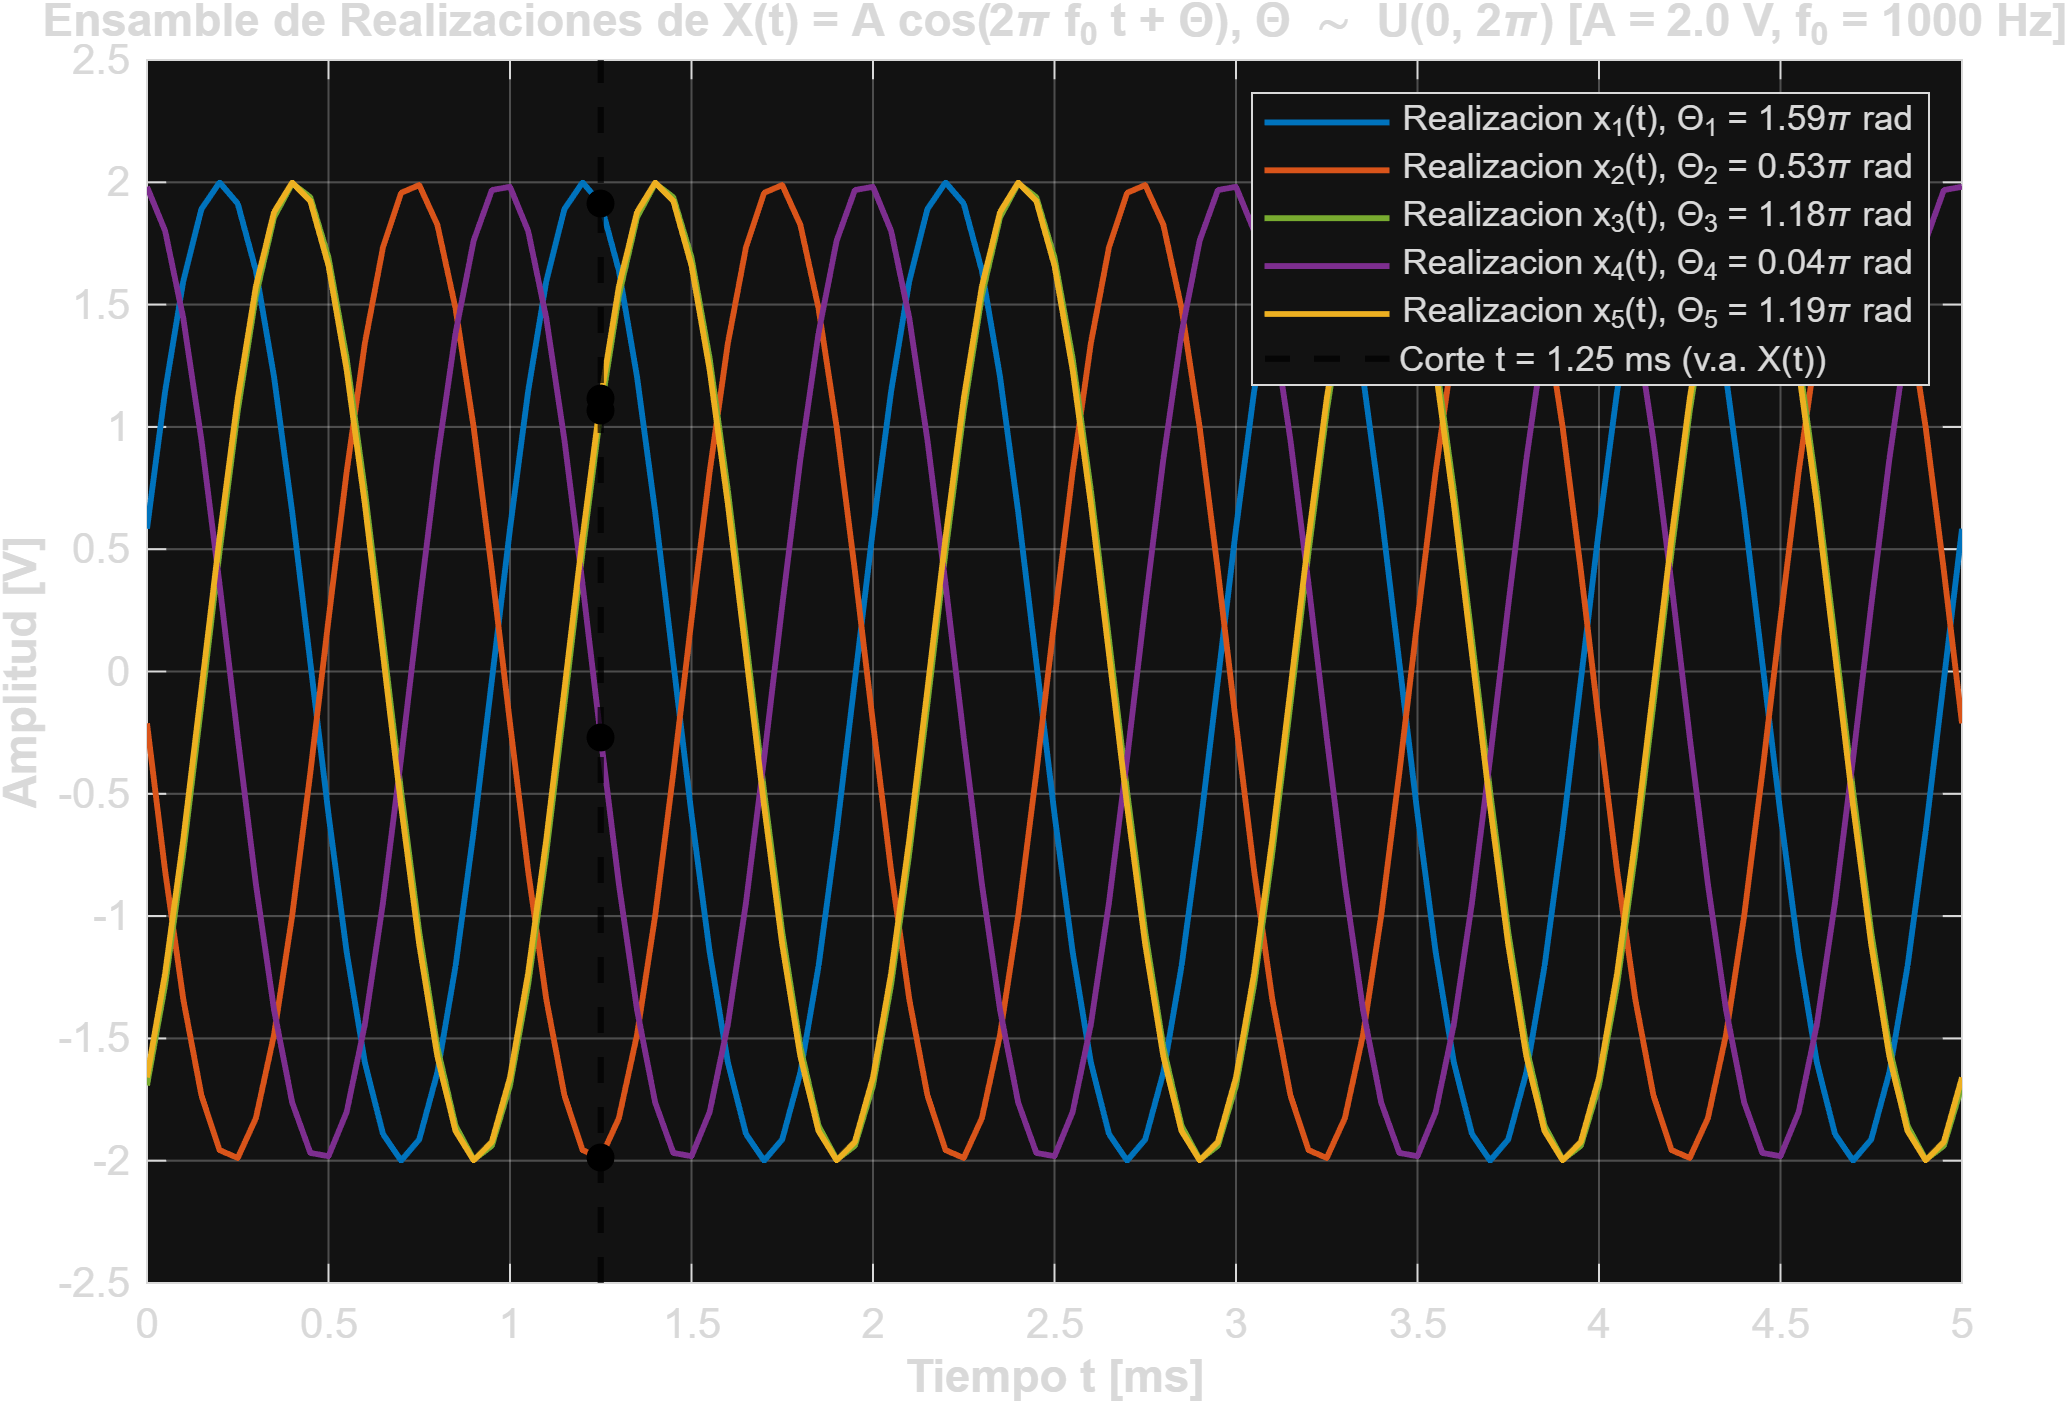
\includegraphics[width=0.98\columnwidth]{figures/fig1_realizaciones_ensamble.png}
\caption{Ensamble de realizaciones del proceso $X(t) = A\cos(2\pi f_0 t + \Theta)$ con $\Theta \sim U(0, 2\pi)$ ($A = 2.0\text{ V}, f_0 = 1000\text{ Hz}$). La línea vertical en $t_0 = 1.25\text{ ms}$ marca el corte transversal que define la variable aleatoria instantánea.}
\label{fig:realizaciones}
\end{figure}

\subsection{Comprobación de Estacionariedad en Sentido Amplio (WSS)}
En la Fig.~\ref{fig:media_var} se presenta la media muestral de conjunto $\hat{\mu}_X(t)$ y la varianza muestral $\hat{\sigma}_X^2(t)$ en función del tiempo para tres tamaños de ensamble: $M \in \{100, 1000, 10000\}$.
\begin{itemize}
    \item \textbf{Media de conjunto:} La curva teórica es idénticamente nula ($\mu_X(t) = 0\text{ V}$). Para $M = 100$, las fluctuaciones estadísticas alcanzan picos de $\pm 0.15\text{ V}$ con un error absoluto medio (MAE) de $0.071433\text{ V}$. Al incrementar el ensamble a $M = 10000$, la media simulada converge notablemente hacia cero en todos los instantes de tiempo, registrando un MAE de apenas $0.011112\text{ V}$.
    \item \textbf{Varianza de conjunto:} La varianza teórica es $R_X(0) = A^2/2 = 2.000000\text{ W}$. La estimación empírica para $M = 10000$ arroja un promedio temporal de $1.999760\text{ W}$, con un error relativo porcentual de únicamente $0.0120\%$. No se observa dependencia funcional del tiempo, confirmando empíricamente la invariancia temporal de segundo orden.
\end{itemize}

\begin{figure}[htbp]
\centering
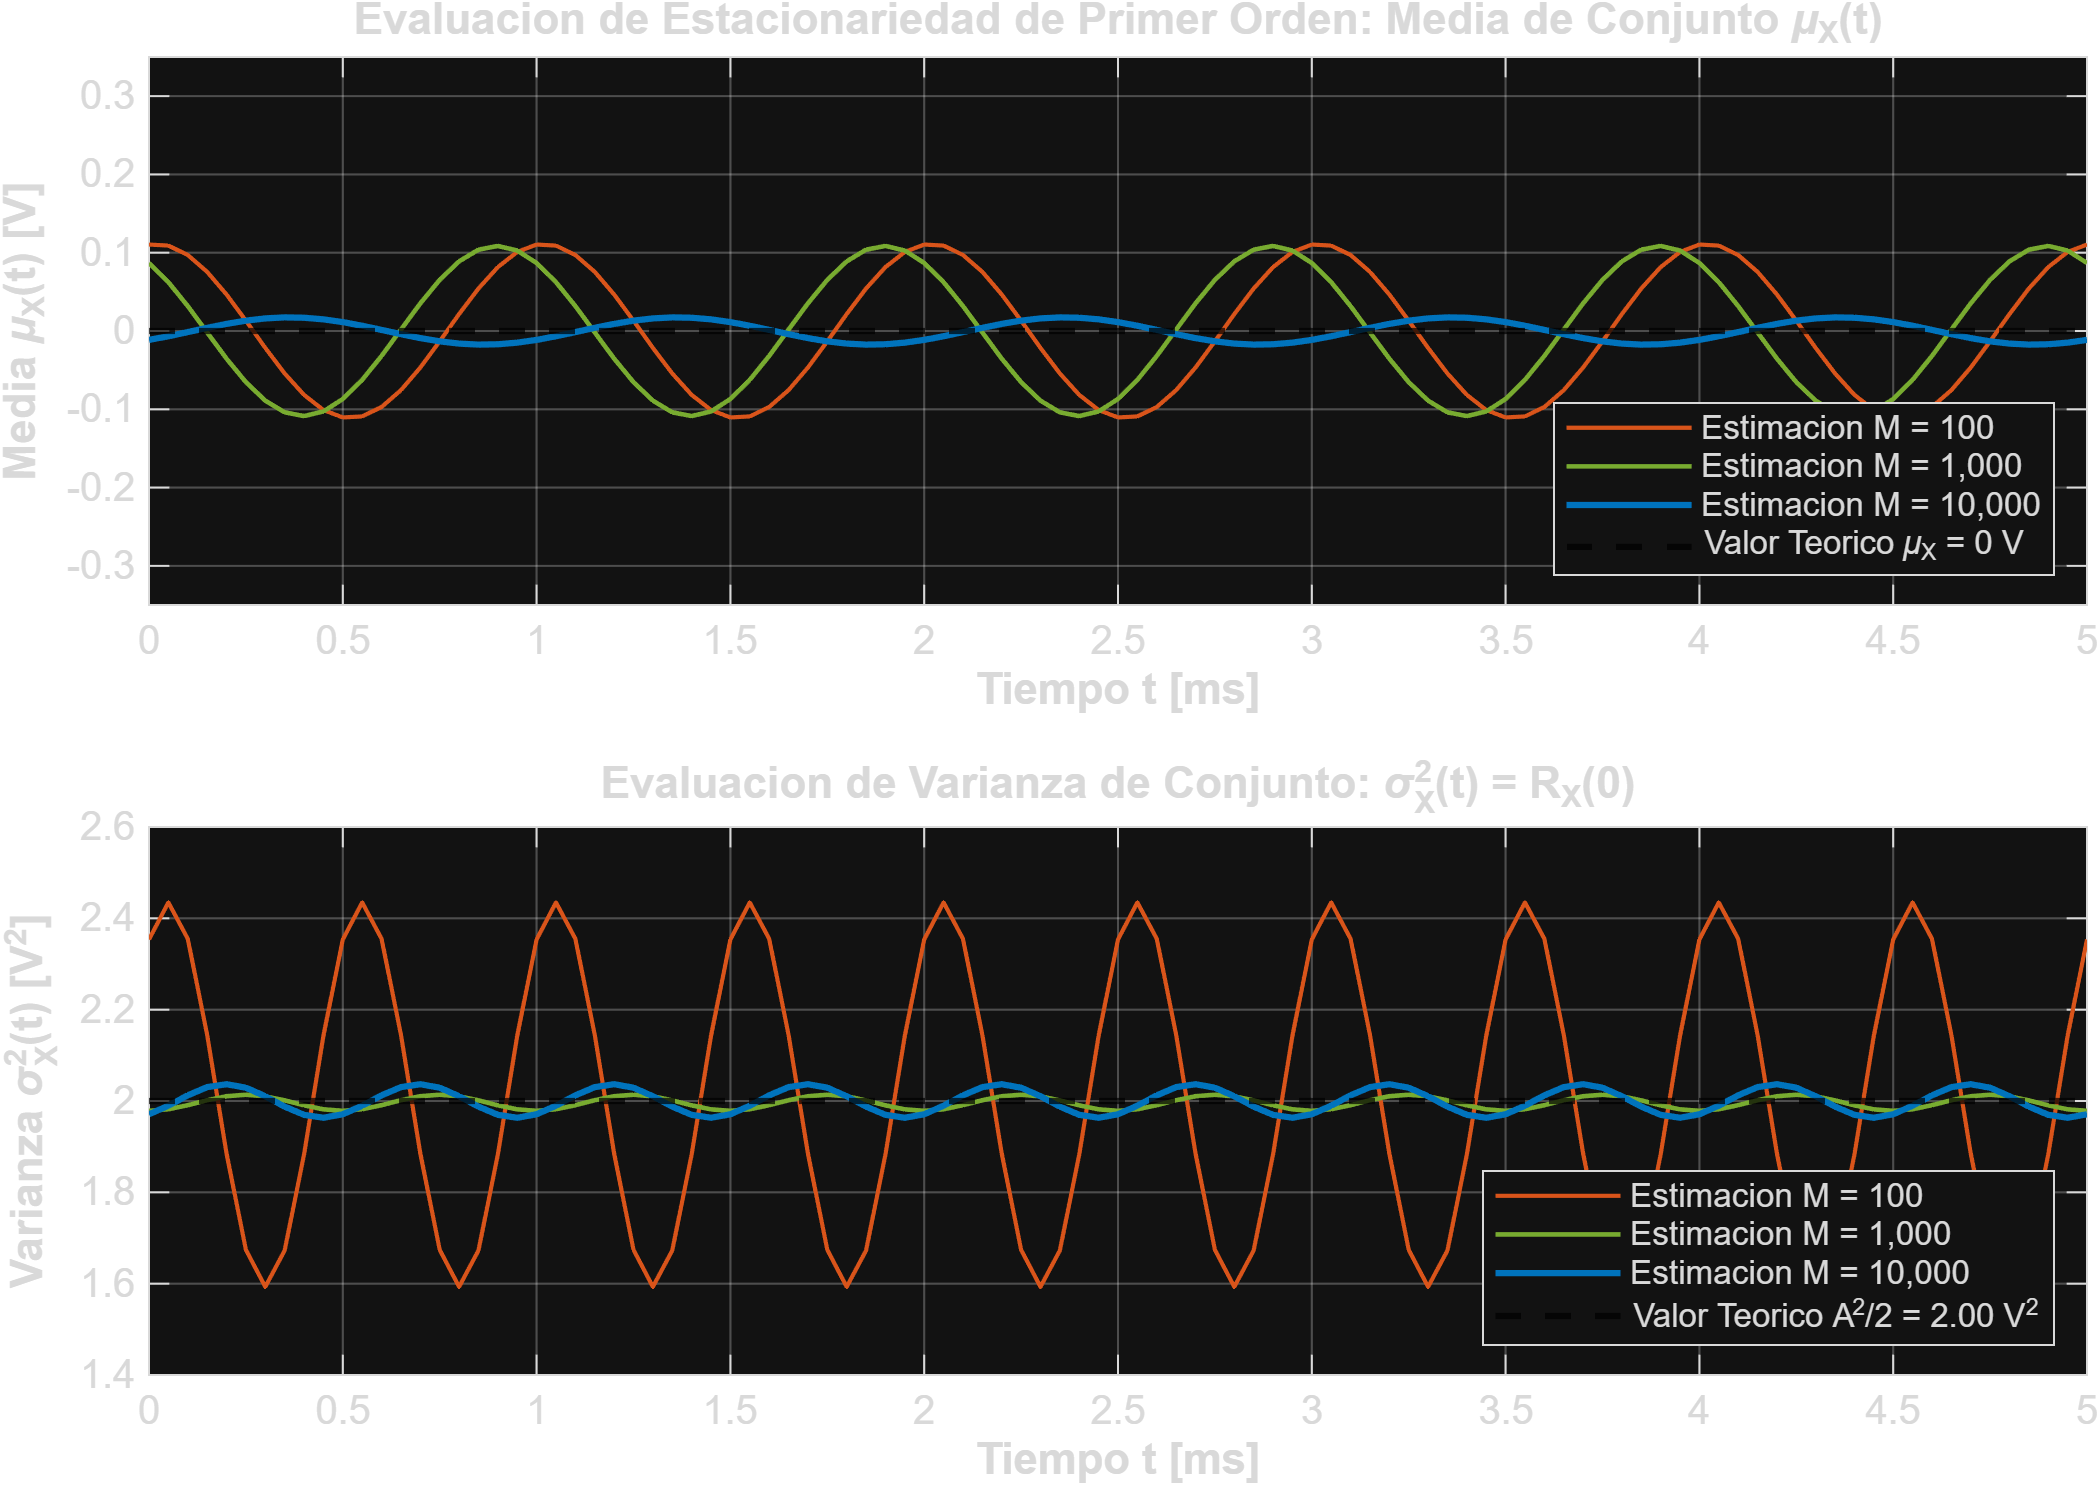
\includegraphics[width=0.98\columnwidth]{figures/fig2_media_y_varianza_conjunto.png}
\caption{Evaluación de estacionariedad de primer y segundo orden. (Arriba) Media de conjunto $\hat{\mu}_X(t)$ frente al valor teórico de 0 V. (Abajo) Varianza de conjunto $\hat{\sigma}_X^2(t)$ frente al valor teórico de $A^2/2 = 2.0\text{ V}^2$.}
\label{fig:media_var}
\end{figure}

La Tabla~\ref{tab:metricas_ensamble} resume cuantitativamente la convergencia de las estadísticas de conjunto a medida que aumenta el número de realizaciones $M$.

\begin{table}[htbp]
\caption{Métricas cuantitativas de conjunto obtenidas en MATLAB.}
\label{tab:metricas_ensamble}
\centering
\resizebox{\columnwidth}{!}{%
\begin{tabular}{rcccc}
\toprule
\textbf{Ensamble $M$} & \textbf{MAE $\hat{\mu}_X(t)$ [V]} & \textbf{RMSE $\hat{R}_X(\tau)$ [W]} & \textbf{$\hat{R}(0)$ [W]} & \textbf{Error Rel. [\%]} \\
\midrule
100    & 0.071433 & 0.073234 & 2.017319 & 0.8660 \\
1,000  & 0.068961 & 0.003416 & 1.995917 & 0.2041 \\
10,000 & 0.011112 & 0.006227 & 1.999760 & 0.0120 \\
\midrule
\textbf{Teórico} & \textbf{0.000000} & \textbf{0.000000} & \textbf{2.000000} & \textbf{0.0000} \\
\bottomrule
\end{tabular}%
}
\end{table}

\subsection{Estructura Bidimensional de la Autocorrelación de Conjunto}
La Fig.~\ref{fig:autocorr} expone en el panel izquierdo la matriz de autocorrelación bidimensional $\hat{R}_X(t_1, t_2)$ calculada con $M = 10000$. En un proceso no estacionario, los valores dependerían de la ubicación absoluta de $(t_1, t_2)$. Sin embargo, la matriz muestra franjas estriadas diagonales homogéneas y perfectamente paralelas a la diagonal principal ($t_1 = t_2$). Esto prueba de manera visual y geométrica que el valor de correlación permanece estrictamente constante para cualquier combinación $(t_1, t_2)$ cuya diferencia $\tau = t_2 - t_1$ sea invariante (estructura de matriz de Toeplitz).

En el panel derecho de la Fig.~\ref{fig:autocorr} se grafica el corte unidimensional $\hat{R}_X(\tau)$ en comparación con la solución analítica $R_X(\tau) = 2\cos(2000\pi \tau)\text{ W}$. La superposición entre la curva analítica (negra continua) y la simulación para $M = 10000$ (azul continua) es prácticamente perfecta en todo el rango de retardos $\tau \in [-5, 5]\text{ ms}$, alcanzando un RMSE de $6.2266 \times 10^{-3}\text{ W}$.

\begin{figure}[htbp]
\centering
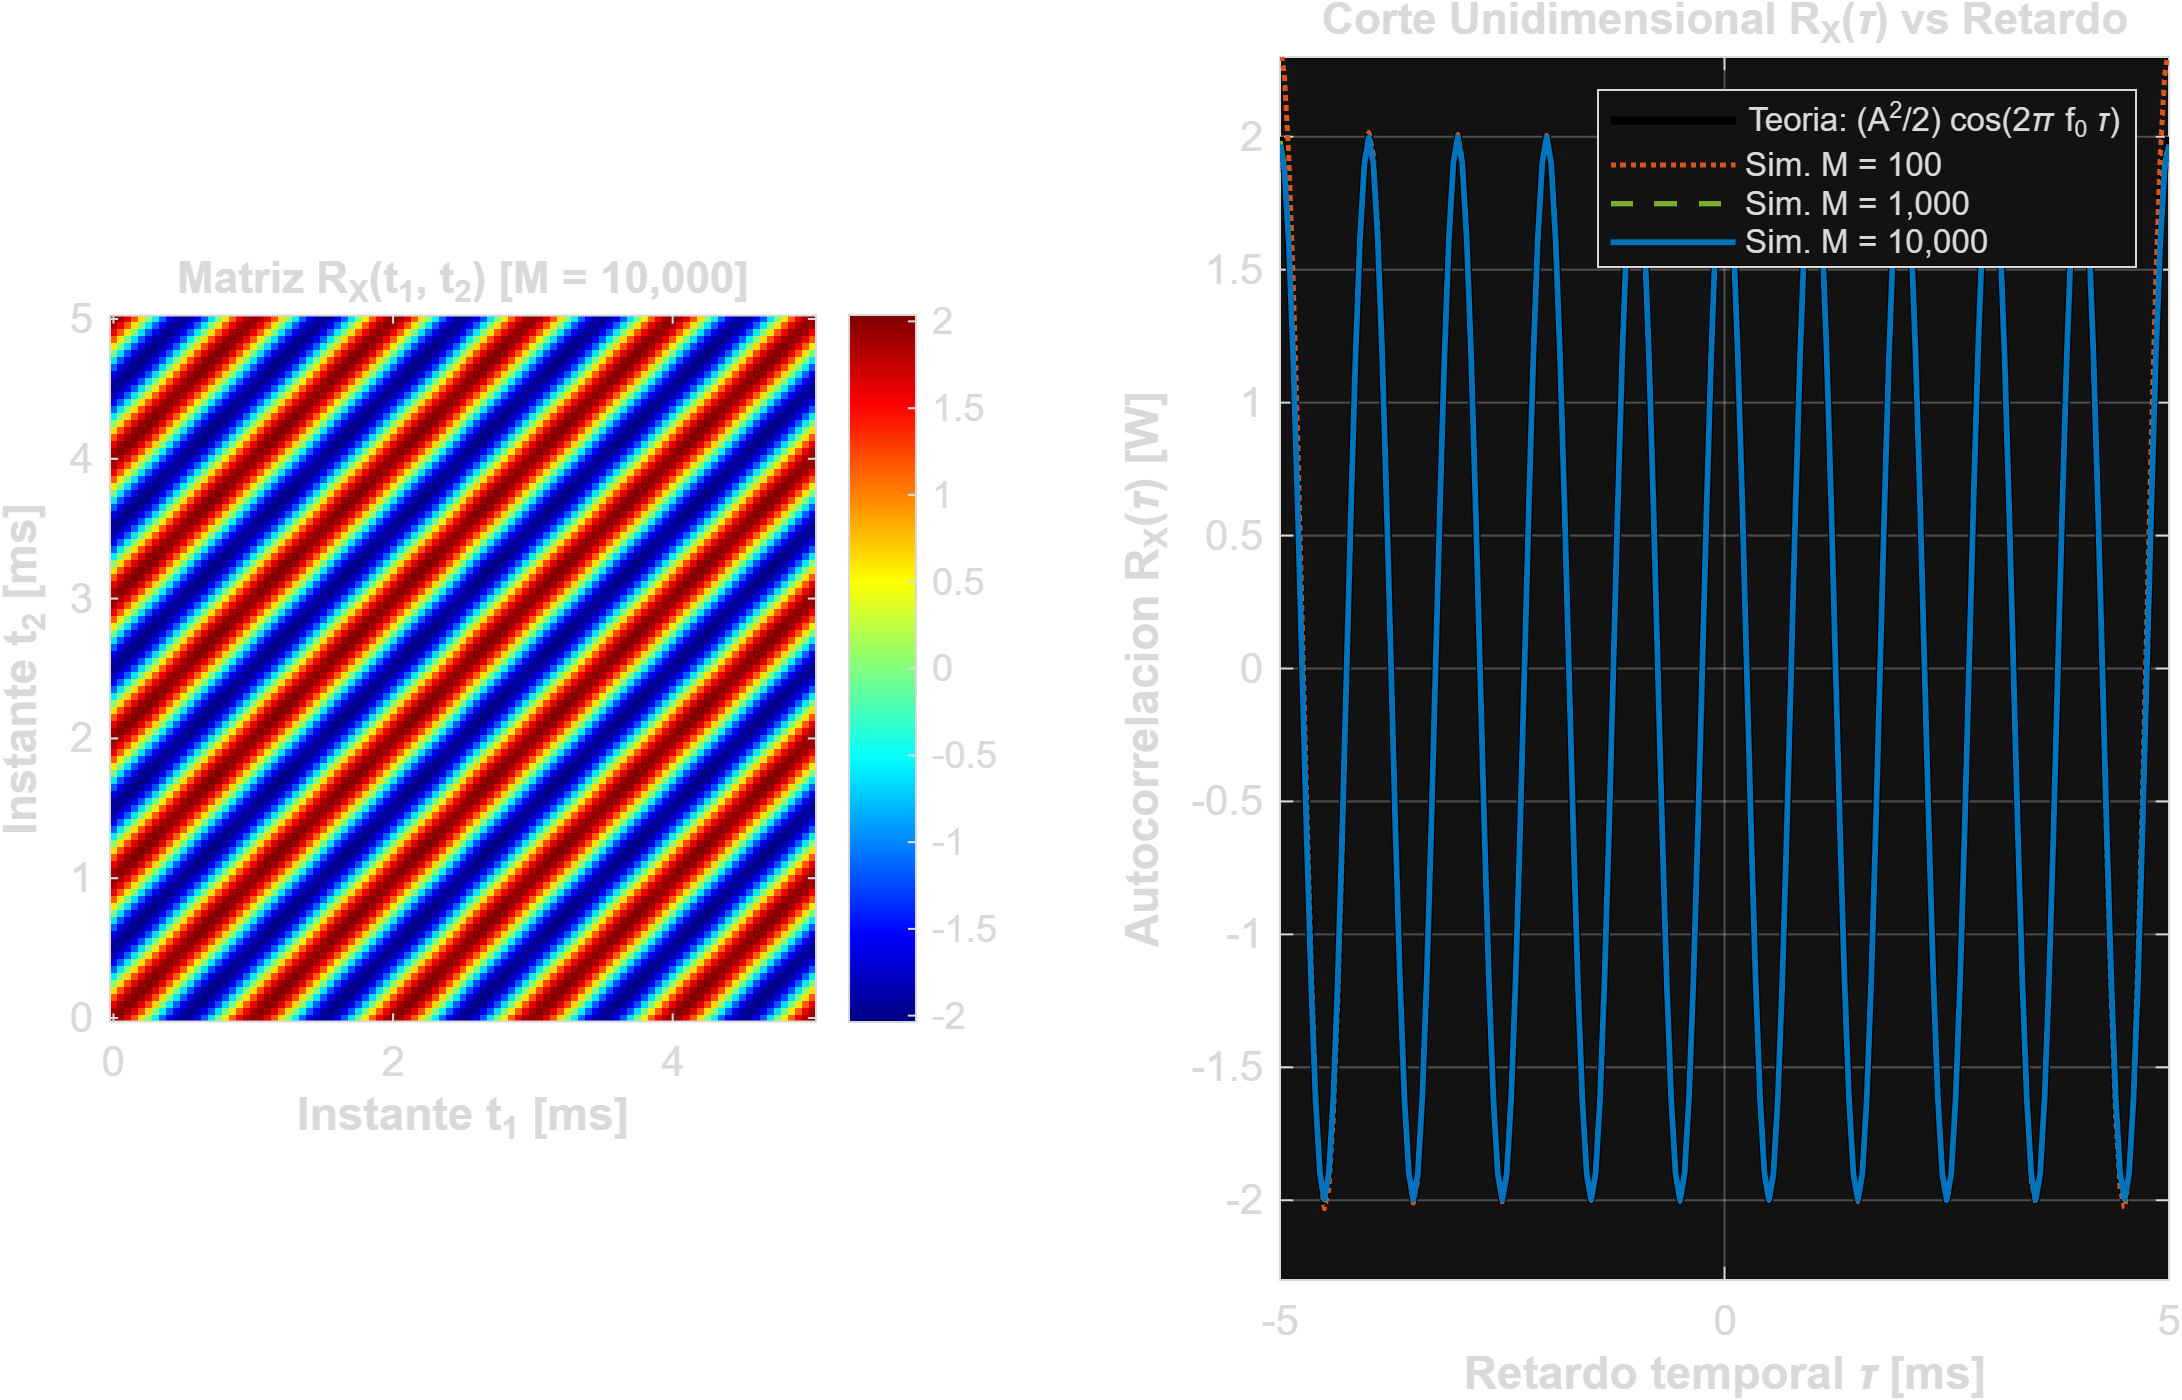
\includegraphics[width=0.98\columnwidth]{figures/fig3_autocorrelacion_conjunto_2d_1d.png}
\caption{Autocorrelación de conjunto. (Izquierda) Matriz bidimensional $\hat{R}_X(t_1, t_2)$ que exhibe simetría diagonal de Toeplitz. (Derecha) Corte unidimensional $\hat{R}_X(\tau)$ contrastado con la curva analítica teórica.}
\label{fig:autocorr}
\end{figure}

\subsection{Validación Experimental de la Ergodicidad}
Para validar la ergodicidad, se tomó una sola realización arbitraria $x_1(t)$ con fase $\Theta_1 = 1.34\pi\text{ rad}$ observada durante $T_{\text{long}} = 1.0\text{ s}$ ($1000$ ciclos de portadora). Se computaron su media y varianza temporal, y su función de autocorrelación temporal $\mathcal{R}_x(\tau)$ mediante el estimador \texttt{xcorr} insesgado.

La Fig.~\ref{fig:ergodicidad} presenta la comparación directa entre la función teórica $R_X(\tau)$, el promedio de conjunto $\hat{R}_{\text{ens}}(\tau)$ con $M = 10000$ realizaciones y el promedio temporal $\mathcal{R}_x(\tau)$ de esa única trayectoria. Como se aprecia en la figura y en la Tabla~\ref{tab:ergodicidad}, la media temporal obtenida es $\langle x(t) \rangle = -1.55065 \times 10^{-5}\text{ V} \approx -0.000016\text{ V}$ (virtualmente cero), y la potencia temporal es de $1.999905\text{ W}$, con un error respecto a la teoría de apenas $0.0048\%$. El RMSE de la autocorrelación temporal frente a la teórica es de apenas $2.17488 \times 10^{-4}\text{ W}$. Esto corrobora empíricamente que una única señal observada a lo largo del tiempo contiene toda la información estadística del ensamble, lo que faculta a los analizadores de espectro en telecomunicaciones para medir la potencia y densidad espectral a partir de un único barrido temporal.

\begin{figure}[htbp]
\centering
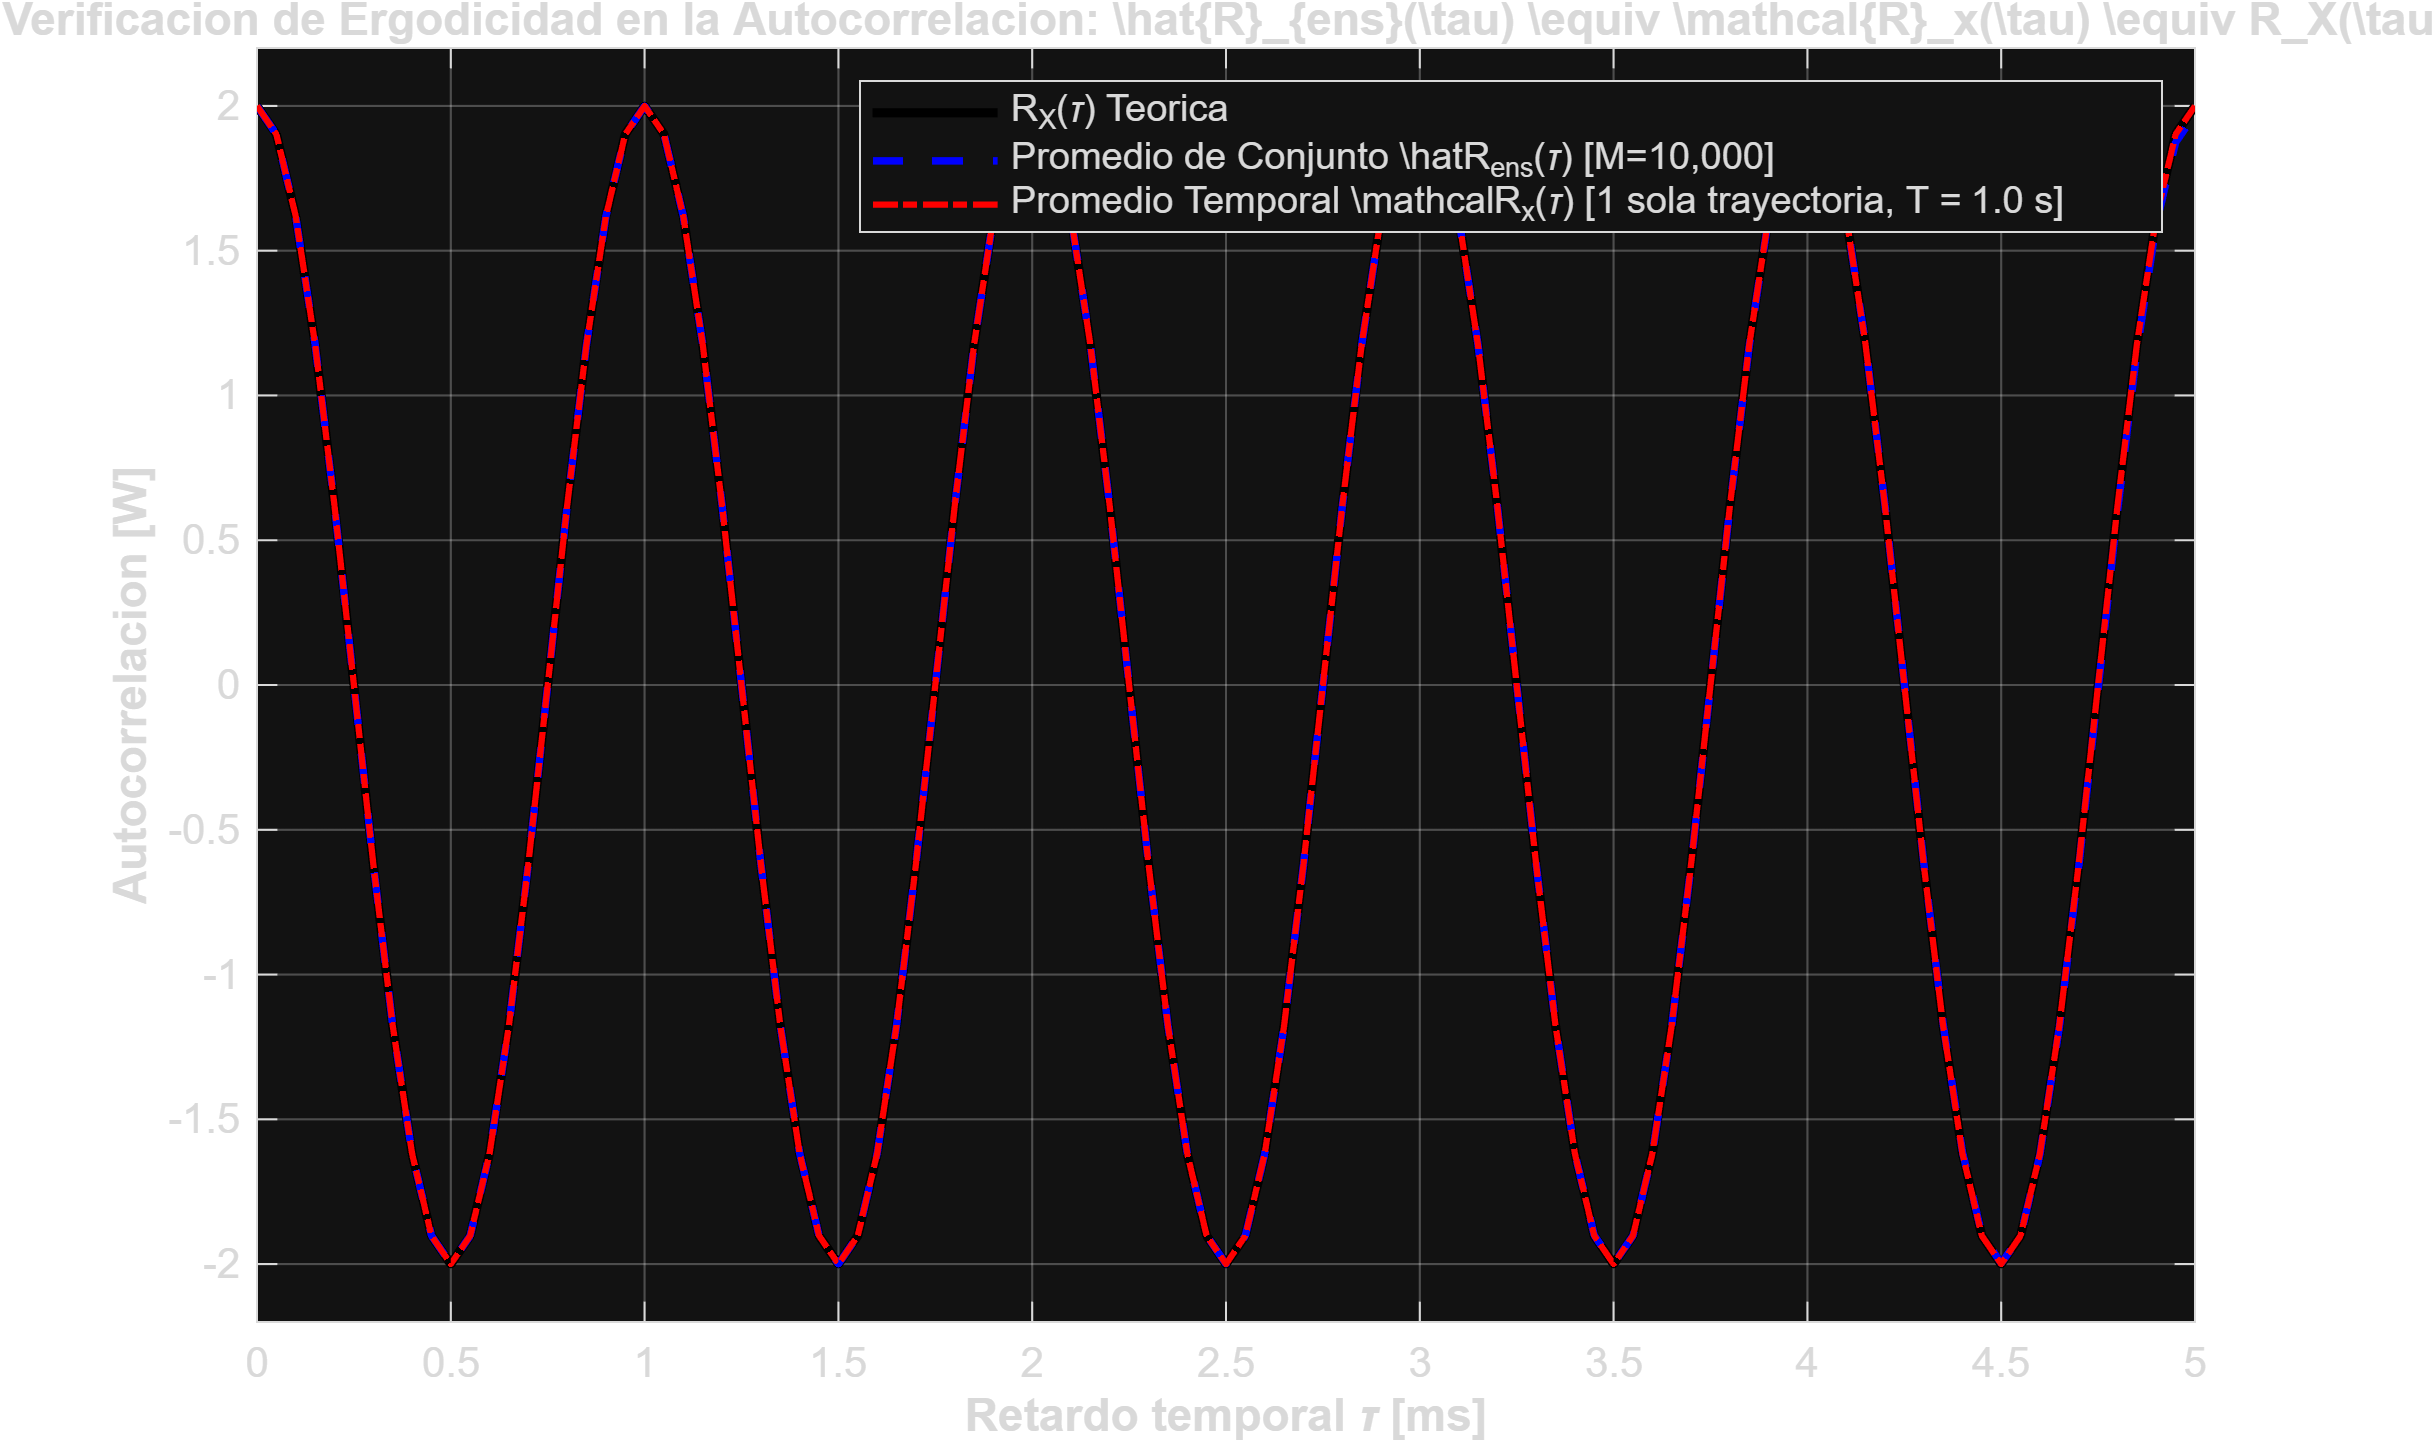
\includegraphics[width=0.98\columnwidth]{figures/fig4_ergodicidad_conjunto_vs_temporal.png}
\caption{Verificación experimental de la ergodicidad en la autocorrelación. La correlación temporal de una sola trayectoria prolongada ($\mathcal{R}_x(\tau)$) coincide con el promedio de conjunto ($\hat{R}_{\text{ens}}(\tau)$) y con la teoría analítica ($R_X(\tau)$).}
\label{fig:ergodicidad}
\end{figure}

\begin{table}[htbp]
\caption{Comparación de promedios de conjunto vs. promedios temporales.}
\label{tab:ergodicidad}
\centering
\resizebox{\columnwidth}{!}{%
\begin{tabular}{lccc}
\toprule
\textbf{Métrica Estadística} & \textbf{Teórico} & \textbf{Conjunto ($M{=}10^4$)} & \textbf{Temporal ($T{=}1\text{ s}$)} \\
\midrule
Media [V] & 0.000000 & 0.011112 & -0.000016 \\
Potencia media $R(0)$ [W] & 2.000000 & 1.999760 & 1.999905 \\
RMSE vs. Teórico [W] & --- & 0.006227 & 0.000217 \\
Error relativo potencia [\%] & 0.0000 & 0.0120 & 0.0048 \\
\bottomrule
\end{tabular}%
}
\end{table}

\subsection{Contraejemplo No Estacionario y Análisis de Fallo}
Para analizar las condiciones de ruptura de la estacionariedad, se modeló el proceso:
\begin{equation}
Y(t) = A (1 + \alpha t) \cos(2\pi f_0 t + \Theta), \quad \alpha = 600\text{ s}^{-1}.
\label{eq:contraejemplo}
\end{equation}
Analíticamente, la media de conjunto de $Y(t)$ sigue siendo nula debido a la periodicidad y uniformidad de $\Theta$: $\mathbb{E}[Y(t)] = 0$. No obstante, su varianza instantánea de conjunto resulta:
\begin{equation}
\sigma_Y^2(t) = \mathbb{E}[Y^2(t)] = \frac{A^2}{2} (1 + \alpha t)^2.
\label{eq:var_contra}
\end{equation}
Asimismo, la autocorrelación de conjunto es:
\begin{align}
R_Y(t_1, t_2) &= \frac{A^2}{2} (1 + \alpha t_1)(1 + \alpha t_2) \nonumber \\
&\quad \times \cos(2\pi f_0 (t_2 - t_1)).
\label{eq:ry_contra}
\end{align}
La presencia del factor multiplicativo dependiente del producto $t_1 \cdot t_2$ rompe la simetría de traslación temporal: la autocorrelación ya no puede expresarse únicamente como función de $\tau = t_2 - t_1$.

\begin{figure}[htbp]
\centering
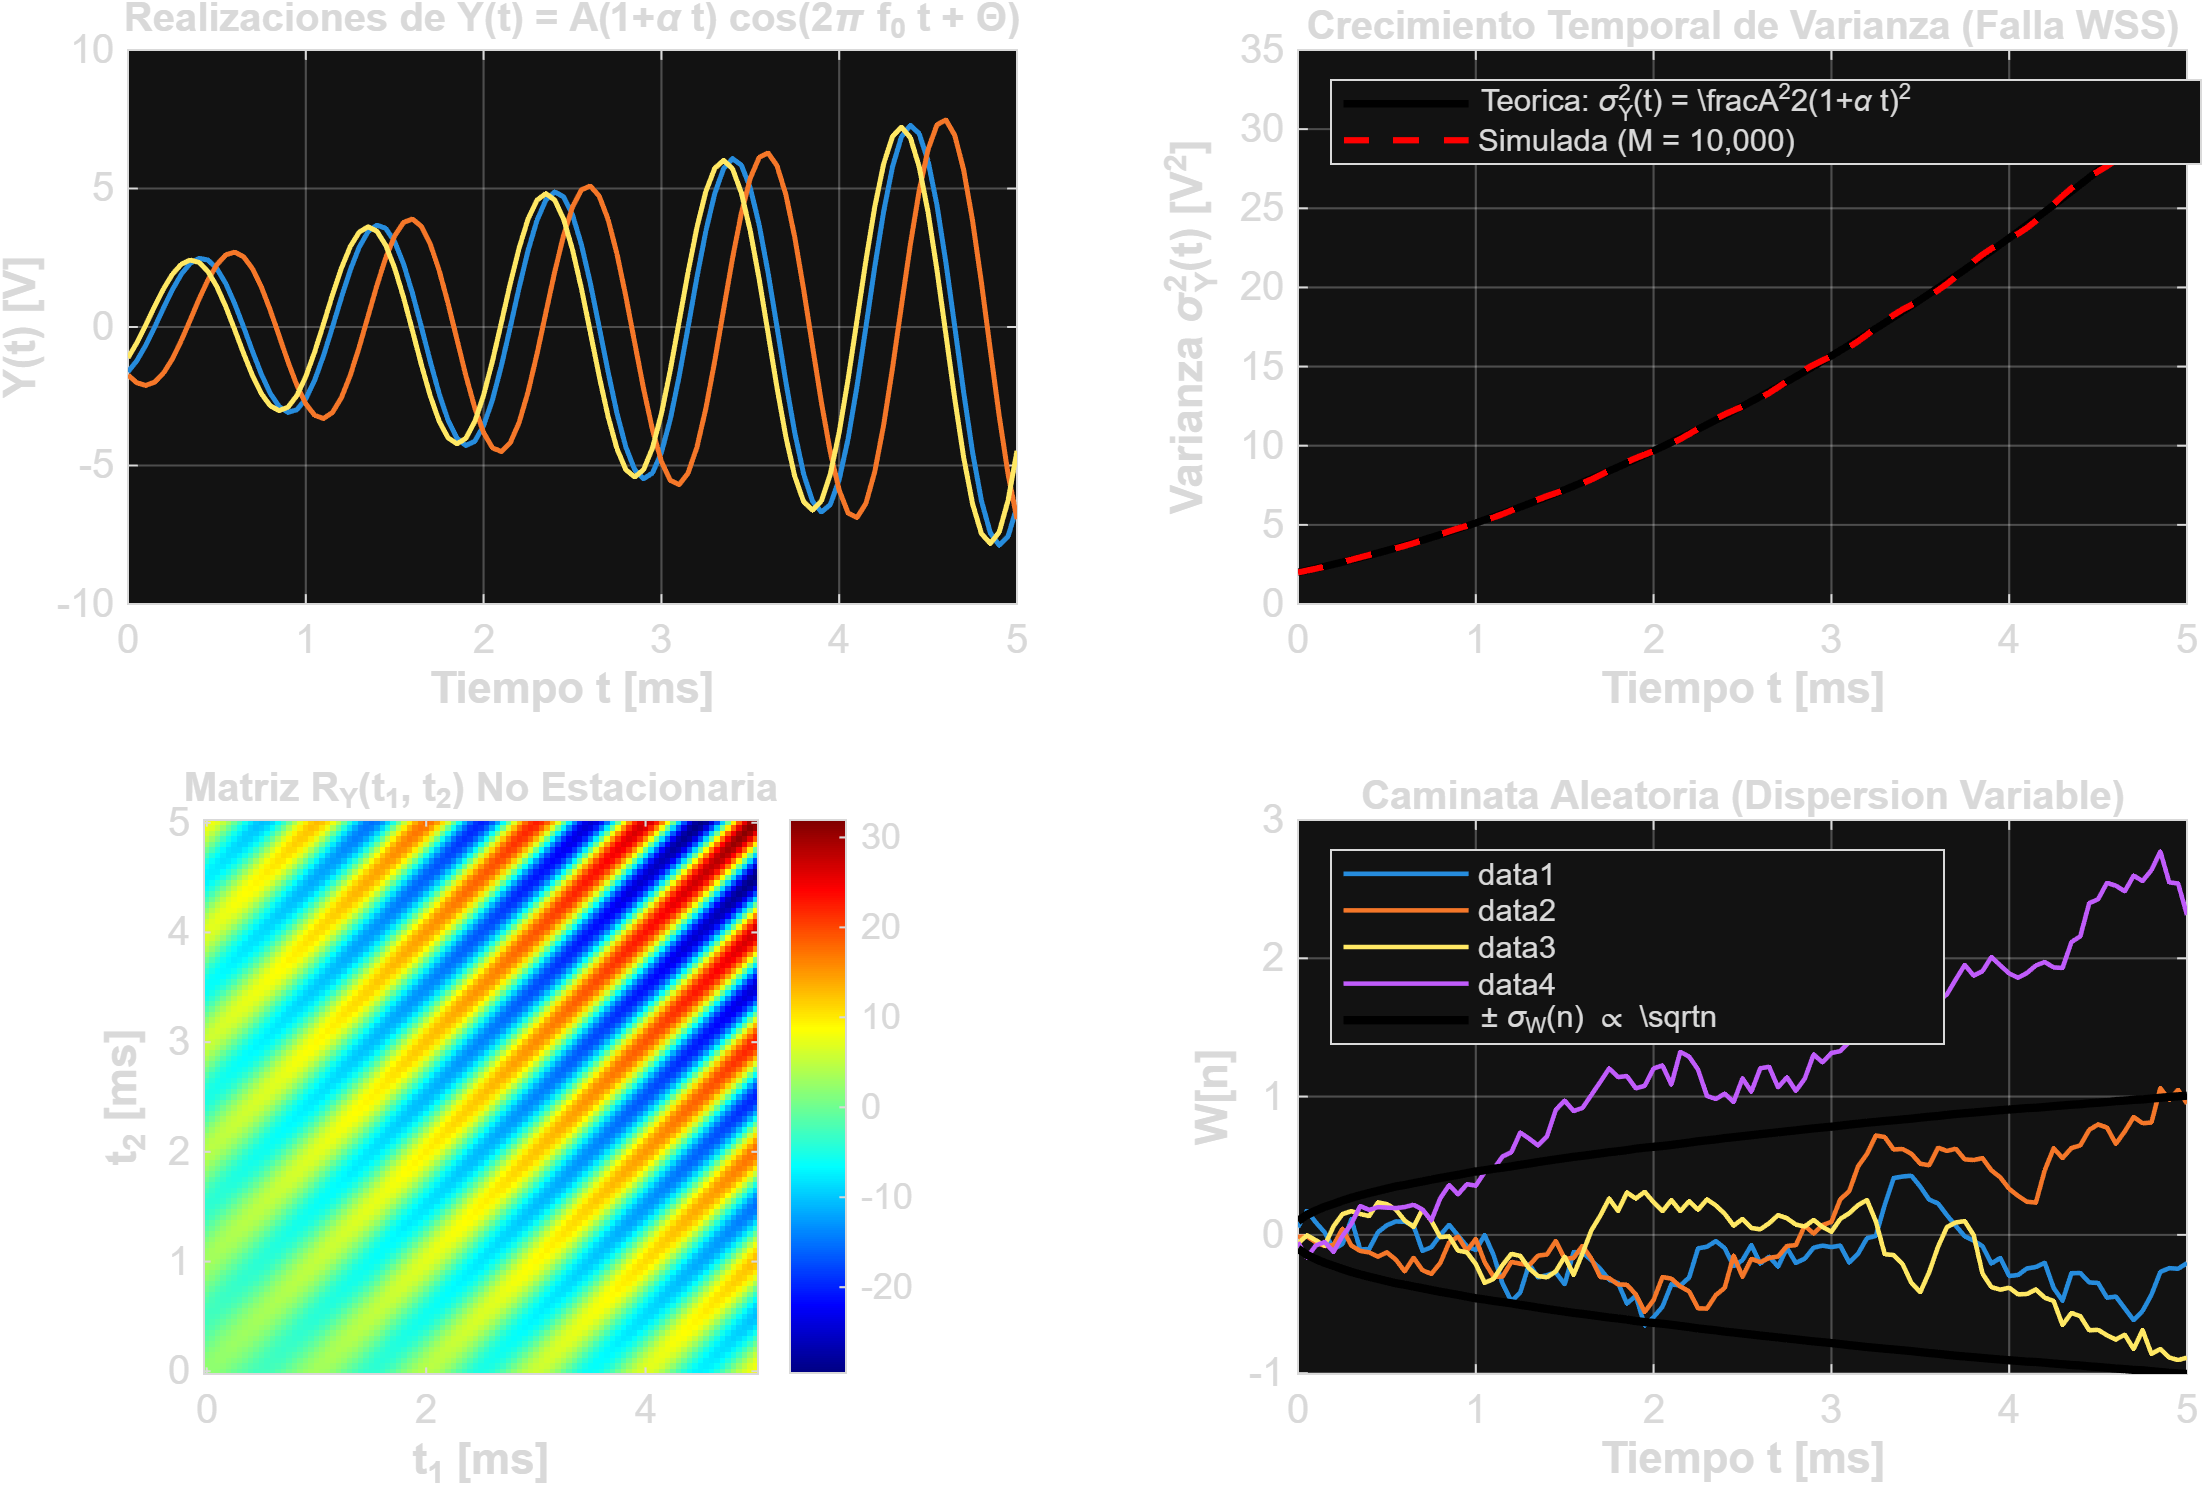
\includegraphics[width=0.98\columnwidth]{figures/fig5_contraejemplo_no_estacionario.png}
\caption{Análisis del contraejemplo no estacionario. (Arriba izq.) Crecimiento de la envolvente de $Y(t)$. (Arriba der.) Varianza temporal cuadrática que invalida WSS. (Abajo izq.) Matriz $R_Y(t_1, t_2)$ asimétrica sin estructura de Toeplitz. (Abajo der.) Caminata aleatoria con dispersión proporcional a $\sqrt{n}$.}
\label{fig:contraejemplo}
\end{figure}

La Fig.~\ref{fig:contraejemplo} evidencia claramente esta violación:
\begin{enumerate}
    \item La envolvente de las trayectorias crece marcadamente en el tiempo (panel superior izquierdo).
    \item La varianza de conjunto (panel superior derecho) se incrementa de forma cuadrática desde $1.996111\text{ W}$ en $t = 0\text{ ms}$ hasta $31.937769\text{ W}$ en $t = 5\text{ ms}$, ajustándose exactamente a la curva teórica (\ref{eq:var_contra}) con un RMSE global de $0.087941\text{ W}$.
    \item La matriz bidimensional $R_Y(t_1, t_2)$ (panel inferior izquierdo) pierde por completo la uniformidad de las bandas diagonales de Toeplitz, concentrando su energía en la esquina superior derecha donde $t_1$ y $t_2$ son máximos.
    \item El panel inferior derecho ilustra una caminata aleatoria discreta $W[n] = \sum_{k=1}^n Z[k]$, cuya dispersión crece como $\sigma_W[n] \propto \sqrt{n}$, análoga a la acumulación de ruido de fase en osciladores locales libres sin lazo de seguimiento PLL (\textit{Phase-Locked Loop}) \cite{demir2000}. En sistemas digitales de alto orden (p.~ej. 1024-QAM en Wi-Fi 7 o 5G-NR), esta no estacionariedad ensancha la línea espectral de la portadora y degrada severamente el diagrama de constelación si no se mitiga con lazos Costas.
\end{enumerate}

\subsection{Convergencia Asintótica de Monte Carlo}
La Fig.~\ref{fig:convergencia} evalúa cuantitativamente la tasa de convergencia de los estimadores empíricos frente al número de trayectorias $M \in [50, 10000]$. En concordancia con el Teorema del Límite Central y la Ley Fuerte de los Grandes Números, los errores decaen a una tasa asintótica proporcional a $1/\sqrt{M}$ (pendiente de $-0.5$ en escala logarítmica). Esto fundamenta el diseño experimental requerido en emuladores de canal de telecomunicaciones para garantizar cotas de error deseadas.

\begin{figure}[htbp]
\centering
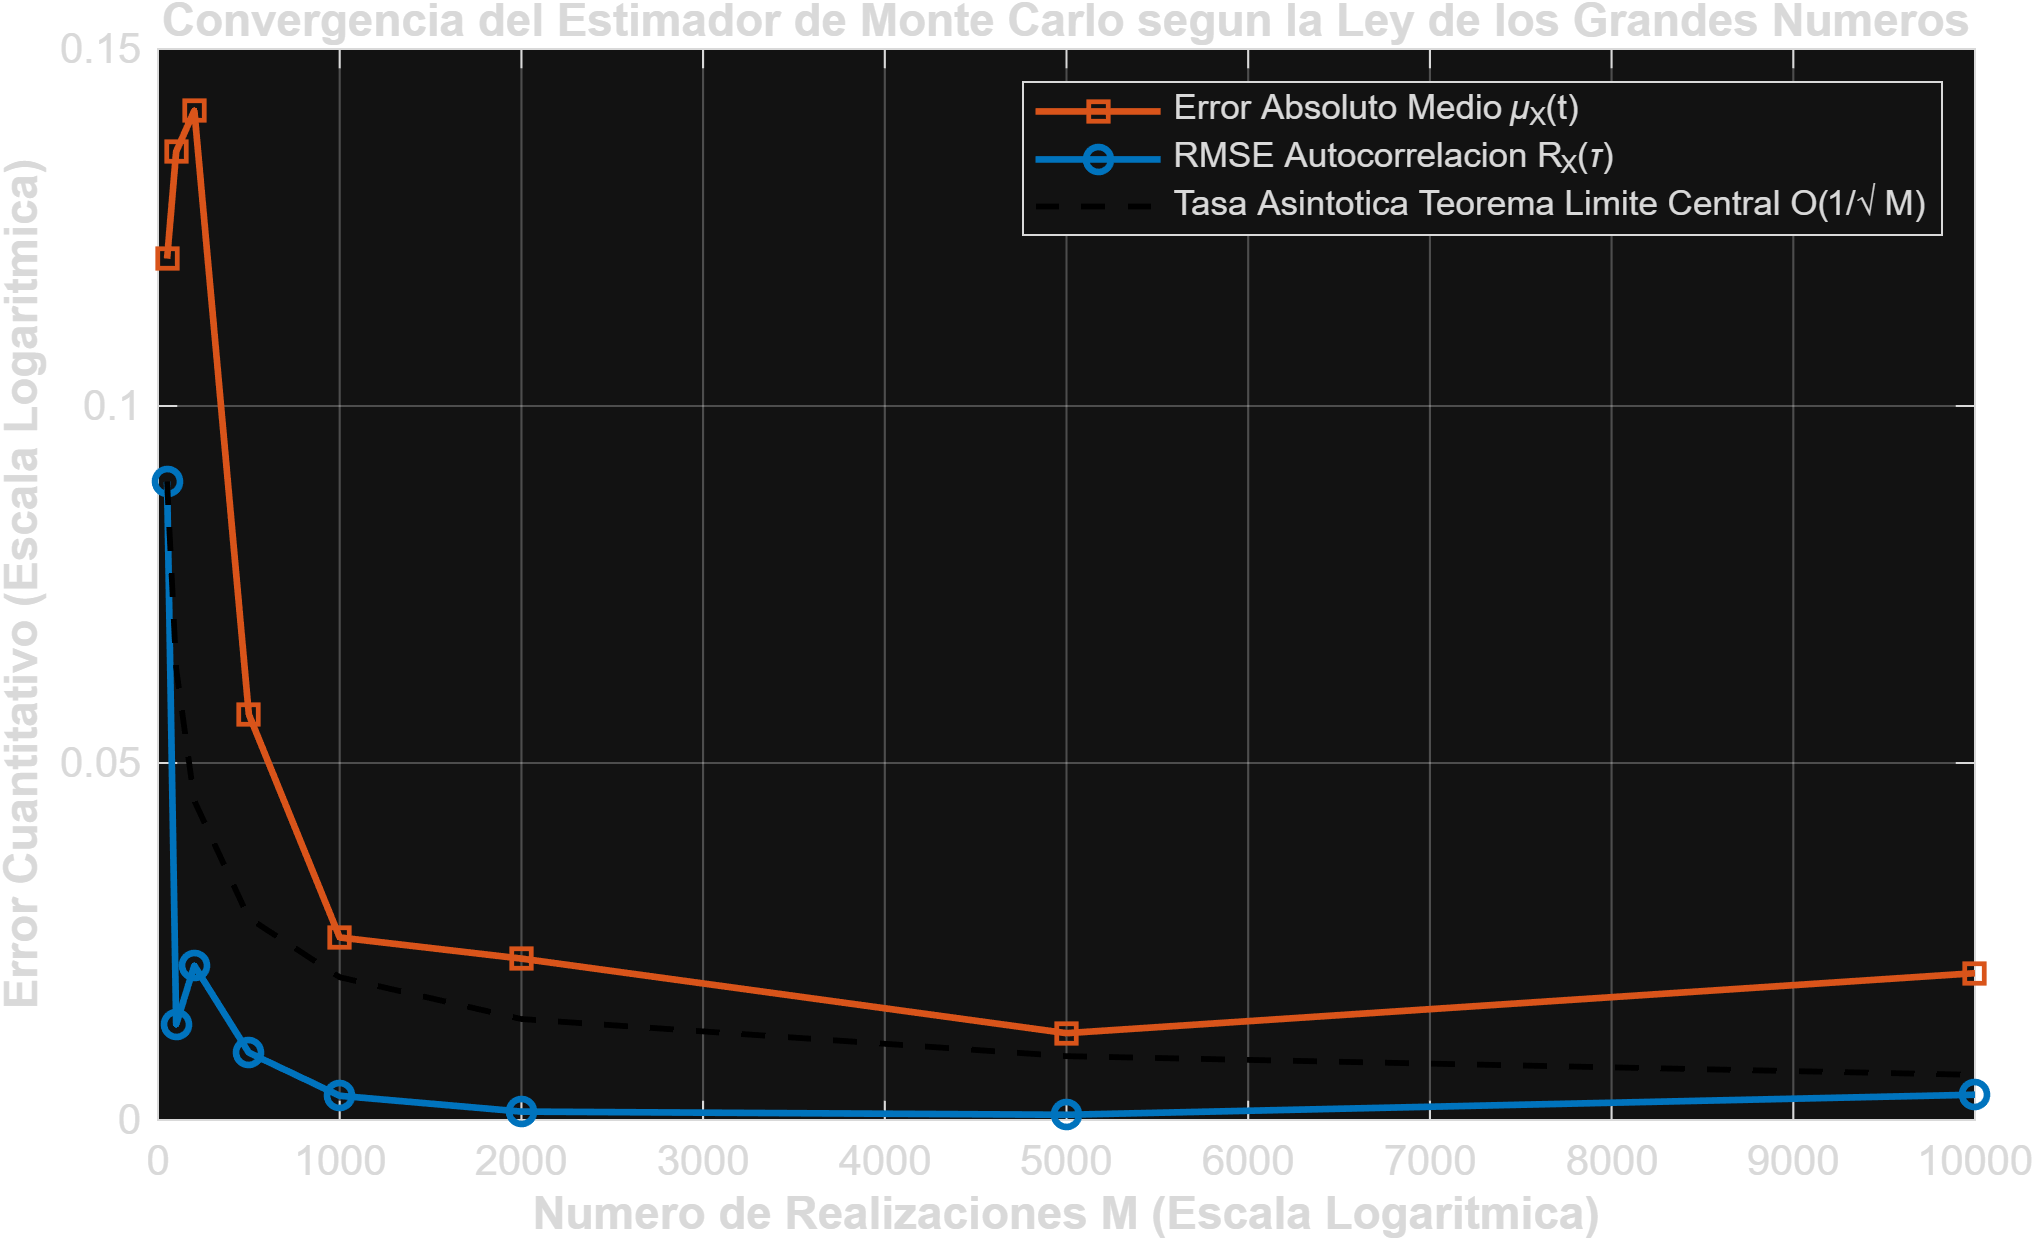
\includegraphics[width=0.95\columnwidth]{figures/fig6_convergencia_monte_carlo.png}
\caption{Convergencia asintótica de los estimadores de Monte Carlo en escala logarítmica, validando la tasa teórica $\mathcal{O}(1/\sqrt{M})$ impuesta por el Teorema del Límite Central.}
\label{fig:convergencia}
\end{figure}

\section{Conclusiones}
\begin{enumerate}
    \item Se dedujo analíticamente y se demostró por simulación en MATLAB que la señal sinusoidal con fase aleatoria $X(t) = A\cos(2\pi f_0 t + \Theta)$ con $\Theta \sim U(0, 2\pi)$ es estrictamente estacionaria en sentido amplio (WSS), dado que su media de conjunto es idénticamente nula ($\mu_X = 0\text{ V}$) y su función de autocorrelación depende únicamente del retardo $\tau$ ($R_X(\tau) = (A^2/2)\cos(2\pi f_0 \tau)$).
    \item El estimador de Monte Carlo validó la potencia media teórica ($2.000000\text{ W}$) con una estimación de $1.999760\text{ W}$ para $M = 10000$ realizaciones, logrando un error relativo porcentual de apenas $0.0120\%$, y ratificando la tasa de convergencia asintótica $\mathcal{O}(1/\sqrt{M})$ predicha por el Teorema del Límite Central.
    \item Se comprobó empíricamente la propiedad de ergodicidad tanto en la media como en la autocorrelación: una única realización evaluada en un intervalo prolongado ($T = 1.0\text{ s}$) reprodujo la función de autocorrelación de conjunto con un RMSE de $2.17488 \times 10^{-4}\text{ W}$ y una potencia temporal de $1.999905\text{ W}$ (error relativo de $0.0048\%$), demostrando la viabilidad operativa de estimar parámetros de procesos estocásticos en analizadores de telecomunicaciones a partir de una única traza temporal.
    \item El análisis del contraejemplo no estacionario $Y(t) = A(1+\alpha t)\cos(2\pi f_0 t + \Theta)$ demostró que la no estacionariedad puede manifestarse preservando la media nula pero rompiendo la invarianza temporal de la varianza (la cual creció de $1.9961\text{ W}$ a $31.9378\text{ W}$) y desestructurando la simetría de Toeplitz en la matriz de autocorrelación $R_Y(t_1, t_2)$.
\end{enumerate}

\begin{thebibliography}{00}
\bibitem{walpole2012}
R.~E. Walpole, R.~H. Myers, S.~L. Myers, y K.~Ye, \emph{Probabilidad y estadística para ingeniería y ciencias}, 9.ª~ed. México: Pearson Educación, 2012.

\bibitem{leon2008}
A.~Leon-Garcia, \emph{Probability, Statistics, and Random Processes for Electrical Engineering}, 3rd~ed. Upper Saddle River, NJ, USA: Pearson/Prentice Hall, 2008.

\bibitem{papoulis2002}
A.~Papoulis y S.~U. Pillai, \emph{Probability, Random Variables and Stochastic Processes}, 4th~ed. New York, NY, USA: McGraw-Hill, 2002.

\bibitem{proakis2008}
J.~G. Proakis y M.~Salehi, \emph{Digital Communications}, 5th~ed. Boston, MA, USA: McGraw-Hill, 2008.

\bibitem{bello1963}
P.~A. Bello, ``Characterization of randomly time-variant linear channels,'' \emph{IEEE Transactions on Communication Systems}, vol.~11, no.~4, pp.~360--393, Dec. 1963.

\bibitem{demir2000}
A.~Demir, A.~Mehrotra, y J.~Roychowdhury, ``Phase noise in oscillators: A unifying theory and numerical methods for characterization,'' \emph{IEEE Transactions on Circuits and Systems I: Fundamental Theory and Applications}, vol.~47, no.~5, pp.~655--674, May 2000.

\bibitem{oppenheim2010}
A.~V. Oppenheim y R.~W. Schafer, \emph{Discrete-Time Signal Processing}, 3rd~ed. Upper Saddle River, NJ, USA: Pearson, 2010.

\bibitem{mathworks_stats}
MathWorks, ``Signal Processing Toolbox and Statistics and Machine Learning Toolbox Documentation,'' The MathWorks, Inc., Natick, MA, USA, 2026. [En línea]. Disponible: \url{https://www.mathworks.com/help/stats/}
\end{thebibliography}

\appendices
\section{Códigos Fuente de MATLAB}
A continuación se presentan los módulos fundamentales implementados para reproducir íntegramente las simulaciones, métricas cuantitativas y figuras del presente artículo. La suite completa consta de 5 funciones modulares, 1 archivo de configuración y 1 script maestro orquestador.

\subsection{Parámetros Globales del Sistema (\texttt{config\_parametros.m})}
\begin{lstlisting}[language=Matlab]
function cfg = config_parametros()
    cfg.seed = 202608;         % Semilla fija
    cfg.A = 2.0;               % Amplitud pico [V]
    cfg.f0 = 1000;             % Frecuencia fundamental [Hz]
    cfg.T0 = 1 / cfg.f0;       % Periodo fundamental [s]
    cfg.fs = 20000;            % Frecuencia de muestreo [Hz]
    cfg.dt = 1 / cfg.fs;       % Intervalo de muestreo [s]
    cfg.T_obs = 5 * cfg.T0;    % Ventana ensamble (5 ms)
    cfg.t = 0:cfg.dt:cfg.T_obs;
    cfg.M_pequeno = 100; cfg.M_medio = 1000; cfg.M_grande = 10000;
    cfg.T_long = 1.0;          % Ventana ergodicidad (1.0 s)
    cfg.t_long = 0:cfg.dt:cfg.T_long;
    cfg.alpha_ramp = 600.0;    % Rampa contraejemplo [s^-1]
end
\end{lstlisting}

\subsection{Generador del Ensamble Sinusoidal con Fase Aleatoria}
\begin{lstlisting}[language=Matlab]
function [X, Theta] = generar_proceso_sinusoidal(M, t, A, f0, seed)
    if nargin >= 5 && ~isempty(seed)
        rng(seed);
    end
    % Muestreo uniforme de la fase Theta ~ U(0, 2*pi)
    Theta = 2 * pi * rand(M, 1);
    
    % Argumento matricial [M x N] para calculo vectorizado
    fase_total = 2 * pi * f0 * t + Theta;
    X = A * cos(fase_total);
end
\end{lstlisting}

\subsection{Estimador de Estadísticas de Conjunto (WSS)}
\begin{lstlisting}[language=Matlab]
function [mu_hat, var_hat, R_mat, R_tau, lags_tau] = estimar_estadisticas_conjunto(X, t)
    [M, N] = size(X);
    % Estimador insesgado de media y varianza de conjunto
    mu_hat = mean(X, 1);
    var_hat = var(X, 0, 1);
    
    % Matriz de autocorrelacion de conjunto: R = (1/M) X' * X
    R_mat = (X' * X) / M;
    
    % Extraccion sobre retardos tau = k * dt
    dt = t(2) - t(1);
    lags_idx = -(N - 1):(N - 1);
    lags_tau = lags_idx * dt;
    R_tau = zeros(1, length(lags_idx));
    for k = 1:length(lags_idx)
        R_tau(k) = mean(diag(R_mat, lags_idx(k)));
    end
end
\end{lstlisting}

\subsection{Estimador de Estadísticas Temporales (Ergodicidad)}
\begin{lstlisting}[language=Matlab]
function [mu_temp, var_temp, R_temp, lags_temp] = estimar_estadisticas_temporales(x_single, t_single, max_lag_sec)
    N = length(x_single);
    dt = t_single(2) - t_single(1);
    % Promedios temporales escalares
    mu_temp = mean(x_single);
    var_temp = var(x_single, 1);
    
    max_lag_samples = round(max_lag_sec / dt);
    % Estimador insesgado mediante xcorr
    [R_raw, lags_idx] = xcorr(x_single, max_lag_samples, 'unbiased');
    R_temp = R_raw;
    lags_temp = lags_idx * dt;
end
\end{lstlisting}

\subsection{Simulación del Contraejemplo No Estacionario}
\begin{lstlisting}[language=Matlab]
function [Y, mu_Y, var_Y, t, R_Y_mat, W, var_W] = simular_contraejemplo(M, t, A, f0, alpha_ramp, seed)
    if nargin >= 6 && ~isempty(seed)
        rng(seed + 100);
    end
    N = length(t);
    Theta = 2 * pi * rand(M, 1);
    
    % Modulacion de amplitud variante en el tiempo
    envolvente = 1 + alpha_ramp * t; 
    fase_total = 2 * pi * f0 * t + Theta;
    Y = (A .* repmat(envolvente, M, 1)) .* cos(fase_total);
    
    mu_Y = mean(Y, 1);
    var_Y = var(Y, 0, 1);
    R_Y_mat = (Y' * Y) / M;
    
    % Caminata aleatoria discreta (ruido de fase acumulado)
    W = cumsum(0.1 * randn(M, N), 2);
    var_W = var(W, 0, 1);
end
\end{lstlisting}

\subsection{Script Orquestador Principal (\texttt{main\_simulacion\_tema08.m})}
\begin{lstlisting}[language=Matlab]
% Flujo maestro de simulacion y generacion de metricas
cfg = config_parametros(); rng(cfg.seed);
% 1. Ensamble de portadora con fase aleatoria
[X_10k, th_10k] = generar_proceso_sinusoidal(cfg.M_grande, cfg.t, cfg.A, cfg.f0, cfg.seed+2);
% 2. Estadisticas de conjunto (WSS)
[mu_10k, var_10k, R_mat, R_tau, lags] = estimar_estadisticas_conjunto(X_10k, cfg.t);
% 3. Ergodicidad: 1 realizacion larga (T = 1.0 s)
[x_l, ~] = generar_proceso_sinusoidal(1, cfg.t_long, cfg.A, cfg.f0, cfg.seed+99);
[mu_t, var_t, R_t, lags_t] = estimar_estadisticas_temporales(x_l, cfg.t_long, cfg.T_obs);
% 4. Contraejemplo no estacionario
[Y, mu_Y, var_Y, ~, R_Y, W, var_W] = simular_contraejemplo(cfg.M_grande, cfg.t, cfg.A, cfg.f0, cfg.alpha_ramp, cfg.seed);
% (Las 6 figuras a 300 DPI se renderizan y guardan automaticamente)
\end{lstlisting}

\end{document}
